%%%%%%%%%%%%%%%%%%%%%%%%%%%%%%%%%%%%%%%%%%%%%%%%%%%%%%%%%%%%%%%%%%%%%%%%%%%%%%%%
%2345678901234567890123456789012345678901234567890123456789012345678901234567890
%        1         2         3         4         5         6         7         8
% THESIS Chapter
\chapter{Data analysis for first and second experiments}
\label{chap:fifth}
\ifpdf
    \graphicspath{{Chapter5/Figures/PNG/}{Chapter5/Figures/PDF/}{Chapter5/Figures/}}
\else
    \graphicspath{{Chapter5/Figures/EPS/}{Chapter5/Figures/}}
\fi

In this section the graphs are displayed, whereas in \ref{chap:conclusions} this will be 
explained. For the second experiment the parsed json structure was used to simplify the 
representation of the data with python.
\section{Results of the first experiment}
The packet structure for the first experiment is as follows:

\begin{minted}{json}
    {
        "powRet": 17,
        "f_port": 42,
        "f_cnt": 51,
        "rssi": -90,
        "rssi_ch": -90,
        "snr": 4.8,
        "bw": 125000,
        "SF": 7,
        "f(MHz)": 867.5,
        "time": "YYY-MM-DDTHH:mm:ss.ssssss+HH:mm",
    }
\end{minted}


The tables for losses on the first experiment are included, but for the second, the tables are on 
 chapter \ref{chap:conclusions} \\
\begin{figure}[htbp]

    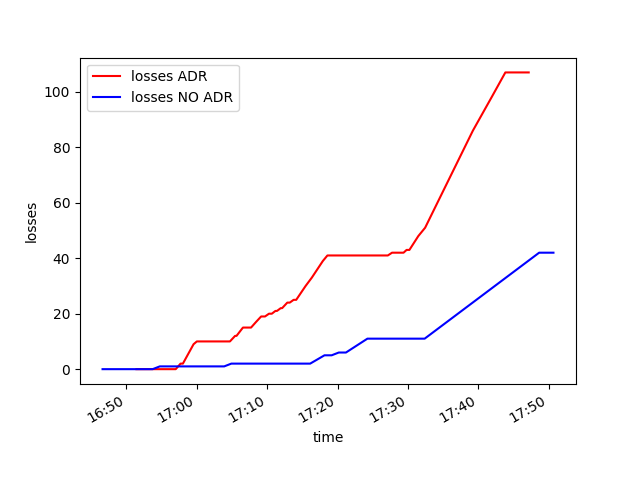
\includegraphics[width=\linewidth]{losses.png}
    \caption{Acummulative packet loss depending on the time the packets arrived}
    \label{chap:fifth:fig:1}
\end{figure}

\begin{figure}[htbp]
    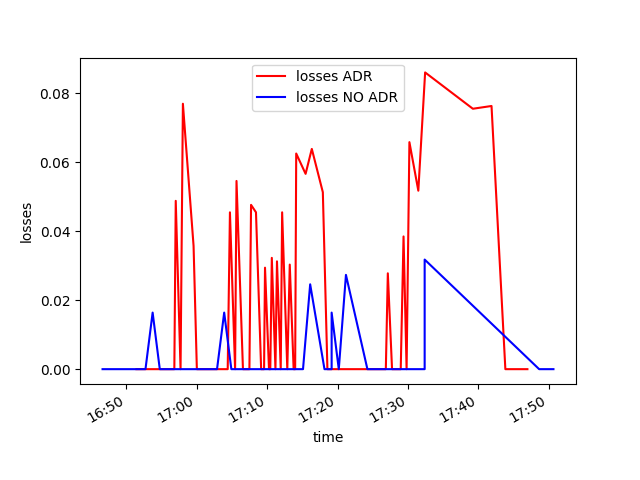
\includegraphics[width=\linewidth]{lossesderivadas.png}
    \caption{The discrete derivative of \ref{chap:fifth:fig:1}}
    \label{chap:fifth:fig:3:noADR}
\end{figure}

\begin{figure}[htbp]
    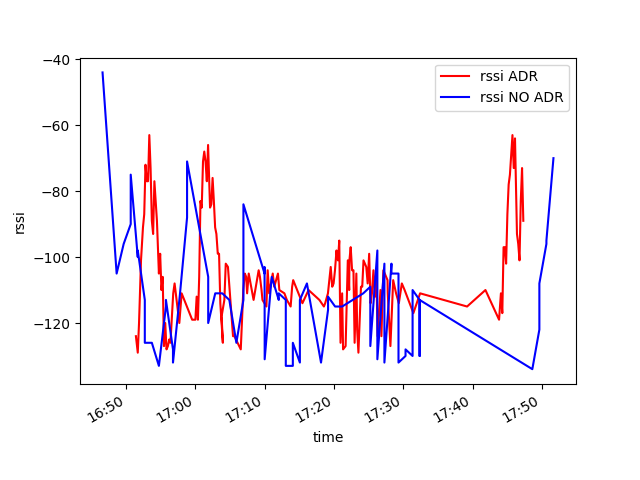
\includegraphics[width=\linewidth]{RSSI.png}
    \caption{RSSI depending on the time}
    \label{chap:fifth:fig:2}
\end{figure}



\begin{table}[htpb]
    \centering
    \setlength{\arrayrulewidth}{0.5mm}
    \setlength{\tabcolsep}{18pt}
    \renewcommand{\arraystretch}{2}
    \begin{tabular}{|c|c|c|c|}
        \hline
         \cellcolor[HTML]{85C1E9}ED configuration & \cellcolor[HTML]{85C1E9}Packets sent & \cellcolor[HTML]{85C1E9}Packets received & \cellcolor[HTML]{85C1E9}Packet loss\\
         \hline
         ADR activated & 263 & 156 & 40.68\% \\
         SF10 and 14 dBm & 112 & 70 & 37.5\% \\
         \hline
    \end{tabular}
    \caption{Table comparing the packet loss of the two cases}
    \label{tab:packet_loss_exp1}
\end{table}

\begin{table}[htbp]
    \centering
    \setlength{\arrayrulewidth}{0.5mm}
    \setlength{\tabcolsep}{18pt}
    \renewcommand{\arraystretch}{2}
    \begin{tabular}{|c|c|c|}
        \hline
         \cellcolor[HTML]{85C1E9}ED configuration & \cellcolor[HTML]{85C1E9}Medium SNR (dB) & \cellcolor[HTML]{85C1E9}Medium RSSI (dBm)\\
         \hline
         ADR activated & 2.07 & -103.68 \\
         SF10 and 14 dBm & -2.11 & -111.85 \\
         \hline
    \end{tabular}
    \caption{Table comparing the medium RSSI and SNR in both cases}
    \label{tab:RSSI_SNR_exp1}
\end{table}


\section{Results of the second experiment}

Our parsed package structure is the following:

\begin{minted}{json}
    {
        "powRet": 17,
        "f_port": 42,
        "f_cnt": 51,
        "rssi": -112,
        "rssi_ch": -112,
        "snr": 4.8,
        "bw": 125000,
        "SF": 7,
        "f(MHz)": 867.5,
        "time": "YYY-MM-DDTHH:mm:ss.ssssss+HH:mm",
        "lat": 44.4134407043457,
        "lng": 8.928983688354492
    }
\end{minted}
This was downloaded and parsed from the storage integration The Things Network provides.
It is suitable for us, since we do not need instant feedback, for that we would have to 
set up a webhook on an external server. The date is on ISO format. 
From here we parse the graphs depicted on chapter \ref{chap:conclusions}.

